\documentclass[12pt]{article}
\usepackage[italian]{babel}
\usepackage{geometry}
\usepackage{amsmath}
\usepackage{amssymb}
\usepackage{graphicx}
\usepackage{ulem}

\geometry{margin=2cm}
\newtheorem{definition}{Definizione}
\newtheorem{example}{Esempio}

\title{Modello Relazionale}
\author{Lorenzo Vaccarecci}
\date{29 Febbraio 2024}

\graphicspath{{../Immagini/}}

\begin{document}
\maketitle
\section{Chiavi}
\textbf{Univocità}: \(X \subseteq \left\{A_{1}, \dots, A_{n}\right\}\) è univoco se qualsiasi sia lo stato di \(R\) non esistono due tuple \(t_{1},t_{2} \in R\) t.c. \(t_{1} \text{ e } t_{2}\) coincidono su \(X\).\\
\textbf{Minimalità}: \(X\) è minimale se nessun \(Y \subsetneq  X\) è univoco.
\begin{example}
    \(\left\{matricola,nome,iseeu\right\}\) è univoco, ma non minimale.
\end{example}
\subsection{Esercizio 1}
\textit{Quali insiemi di attributi soddisfano la proprietà di univocità rispetto a questa istanza di relazione?}
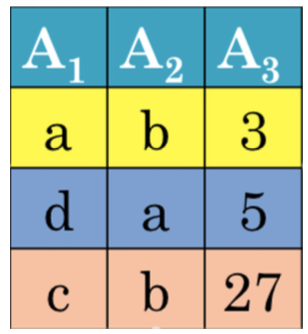
\includegraphics[width=5cm]{esercizio2.png}
Dipende, ma \(A_{2}\) non è univoco, mentre \(A_{1}\) e \(A_{3}\) lo sono.
\subsection{Esercizio 2}
\textit{Se \(\left\{A,B\right\}\) soddisfa la proprietà di univocità quali delle seguenti \textbf{possono} essere chiavi?}\\
Opzioni:
\begin{itemize}
    \setlength\itemsep{0em} 
    \item \(\left\{A\right\}\)
    \item \(\left\{A,B,C\right\}\)
    \item \(\left\{C\right\}\)
    \item \(\left\{C,D\right\}\)
    \item \(\left\{C,D,E\right\}\)
\end{itemize}
Risposta: tutte tranne \(\left\{A,B,C\right\}\)
\subsection{Esercizio 3}
\begin{center}
    \makebox[\textwidth]{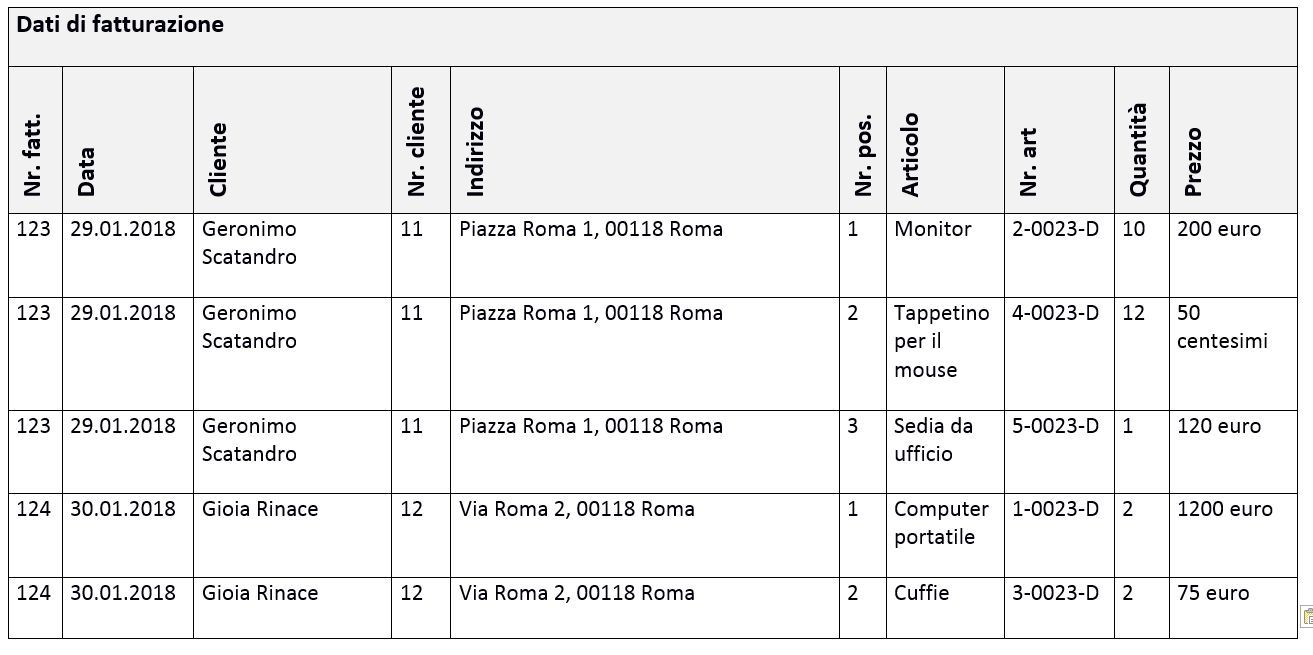
\includegraphics[width=0.8\paperwidth]{esercizio3.jpg}}
\end{center}
\textit{Quali chiavi individuereste per questa relazione? (non basarsi solo sull'istanza corrente)}\\
Risposta:
\begin{itemize}
    \setlength\itemsep{0em} 
    \item Nr.fattura + Nr.pos (Non avremmo mai due righe con lo stesso numero di fattura e posizione)
    \item Nr.fattura + Nr.art (Non avremmo mai due righe con lo stesso numero di fattura e articolo)
\end{itemize}
\subsection{Tipi di chiave}
\begin{itemize}
    \setlength\itemsep{0em} 
    \item \textbf{Chiave candidata}: tutte le possibili chiavi
    \begin{itemize}
        \item \textbf{Chiave primaria}: scelta tra le chiavi candidate in modo da effettuare efficientemente ricerche (non può essere nulla), la indichiamo con \(\underline{A}\)
        \item \textbf{Chiave alternativa}: chiave candidata non scelta come chiave primaria, la indichiamo con \(\uwave{A}\)
        \item \textbf{Superchiave}: univoca e non minimale
    \end{itemize}
\end{itemize}
\begin{example}
    Studente(\uline{matricola}, nome, cognome , dataNascita, \uwave{codiceFiscale}, tipoDiploma, annoDiploma, votoDiploma, iseeu\(_{o}\), media, relatore, annoIscrizione)
\end{example}
\subsubsection{Esercizio 4}
NOLEGGIO(colloc, dataNol, cliente, dataRest\(_{o}\))\\
\textit{Trovare gli insiemi univoci e le chiavi.}\\
Risposta:
\begin{itemize}
    \setlength\itemsep{0em}
    \item \(\left\{colloc, dataNol\right\} \rightarrow\) NOLEGGIO(\uline{colloc}, \uline{dataNol}, cliente, dataRest\(_{o}\))
    \item \(\left\{colloc, dataRest_{o}\right\} \rightarrow\) non posso usarla come chiave, perchè non può essere opzionale
\end{itemize}
\end{document}